\section{Related Work}
\label{sec:related}

\begin{figure}[!t]
    \centering
    
\includegraphics[width=0.175\textwidth]{walker_task.png}
    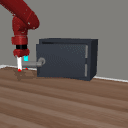
\includegraphics[width=0.175\textwidth]{dooropen_task.png}
    \vspace{-0.2cm}
    \caption{\footnotesize Visualization of our image-based environments. The observations are $64\times 64$ and $128\times 128$ raw pixel images for the \texttt{walker-walk} and \texttt{sawyer-door} tasks respectively. The \texttt{sawyer-door-close} environment used in our generalization experiments in Section~\ref{sec:generalization_exps} also uses the same environment as \texttt{sawyer-door}.}
    \label{fig:visual}
    \vspace{-0.6cm}
\end{figure}

Offline RL~\citep{ernst2005tree, riedmiller2005neural, LangeGR12, levine2020offline} is the task of learning policies from a static dataset of past interactions with the environment. It has found applications in domains including robotic manipulation~\citep{ kalashnikov2018scalable, mandlekar2020iris, Rafailov2020LOMPO,singh2020cog}, NLP~\citep{jaques2019way,jaques2020human} and healthcare~\citep{shortreed2011informing, Wang2018SupervisedRL}. Similar to interactive RL, both model-free and model-based algorithms have been studied for offline RL, with explicit or implicit regularization of the learning algorithm playing a major role.

%%SL.1.23: would be good to cite older batch RL work (see my tutorial article), as well as add some citations to more applied work that uses offline/batch RL.
%%TY.1.26: I added those citations in the above paragraph.

% \textbf{Model-free offline RL} Prior model-free algorithms have employed techniques including regularized variants of importance sampling based policy learning~\citep{precup2001off, sutton2016emphatic, LiuSAB19, SwaminathanJ15, nachum2019algaedice}; offline actor-critic methods~\citep{siegel2020keep, peng2019advantage}; applying uncertainty quantification to the predictions of the Q-values~\citep{agarwal2020optimistic, kumar2019stabilizing, wu2019behavior, levine2020offline}, or learning conservative Q-values~\citep{kumar2020conservative}. A second class of algorithmns


\textbf{Model-free offline RL.} Prior model-free offline RL algorithms have been designed to regularize the learned policy to be ``close`` to the behavioral policy either implicitly via regularized variants of importance sampling based algorithms~\citep{precup2001off, sutton2016emphatic, LiuSAB19, SwaminathanJ15, nachum2019algaedice}, offline actor-critic methods~\citep{siegel2020keep, peng2019advantage}, applying uncertainty quantification to the predictions of the Q-values~\citep{agarwal2020optimistic, kumar2019stabilizing, wu2019behavior, levine2020offline}, and learning conservative Q-values~\citep{kumar2020conservative} or explicitly measured by direct state or action constraints~\cite{fujimoto2018off,liu2020provably},
KL divergence~\citep{jaques2019way,wu2019behavior, zhou2020plas}, Wasserstein distance, and MMD~\citep{kumar2019stabilizing}. 
%%CF: This paper is also missing: https://arxiv.org/abs/2011.07213
%%TY.2.3: added it to the family of using KL as the policy constraint.
% While these methods provide a number of ways to regularize the policy or value function to mitigate distributional shift, they typically require the learned policy to stay close to the data~\citep{levine2020offline} and could be too conservative when the dataset is diverse and contains substantial suboptimal examples.
%%SL.1.23: This seems like it's tarring a wide range of prior work with a very broad brush... maybe we can tone this down a bit. I think reviewers are likely to object to some of these statements and we wouldn't really have the evidence to back it up
%%TY.1.26: I toned it down a bit.
%%CF: I think it's still pretty aggressive. Can you instead be positive about the potential of our approach in contrast to these? (e.g. Unlike these prior methods, we ...")
%%SL.1.31: I actually think this discuss more generally is hard to parse -- but I also don't think we entirely need it. I would suggest just deleting the above sentence, and replacing it instead with a discussion of conservatism. Maybe Aviral can suggest some citations, but in terms of phrasing, we can say something like this: While these methods provide a number of ways to regularize the policy or value function to mitigate distributional shift, they typically require the learned policy to stay close to the data.
%%TY.2.3: I took Sergey's suggested phrasing with references to the offline RL tutorial (Aviral can correct this if it's not appropriate) and added one more sentence to emphasize that model-free methods do not optimize generalization abilities.
Different from these works, COMBO uses both the offline dataset as well as simulated data from a learned dynamics model. This allows COMBO to behave less conservatively by optimizing a tighter lower bound of policy performance, as well as gain broader generalization when the model bias is small, as demonstrated through our theoretical analysis and experiments.
%%SL.1.31: I'm torn about this conservatism thing. I do believe it's true, but I'm not sure we have evidence to back this up. In the absence of evidence, we could consider toning down these conservatism claims. The reason I'm concerned about it is that it's very easy for a reviewer to say: all this model-based stuff relies on the data just like model-free, so there is no reason to expect it to generalize better.
%%TY.2.3: I think our theory section shows that COMBO achieves a tighter lower bound and thus is less conservative and the generalization experiments also show that COMBO generalizes better than CQL. I included references to those two sections.

\textbf{Model-based offline RL.} Model-based offline RL methods~\citep{finn2017deep, ebert2018visual, kahn2018composable, kidambi2020morel, yu2020mopo, matsushima2020deployment, argenson2020model, swazinna2020overcoming,Rafailov2020LOMPO, lee2021representation} provide an alternative approach to policy learning that involves the learning of a dynamics model using techniques from supervised learning and generative modeling. Such methods however rely either on uncertainty quantification of the learned dynamics model which can be difficult for deep network models~\cite{ovadia2019can}, or on directly constraining the policy towards the behavioral policy similar to model-free algorithms~\cite{matsushima2020deployment}. In contrast, COMBO conservatively estimates the value function by penalizing it in out-of-support states generated through model rollouts. This allows COMBO to retain all benefits of model-based algorithms such as broad generalization, without the constraints of explicit policy regularization or uncertainty quantification.
%%SL.1.23: I don't think this is a statement that we can really back up, it's not clear why (or even if) model-based methods would be any better for generalizing beyond the support of the data. It would be nice to work in some older citations too (see the offline RL tutorial), otherwise it kind of creates the impression that running model-based RL on logged data was invented in 2020, which it most definitely wasn't. 
%%TY.1.26: I changed the benefit of MBRL to the advantage of using supervised learning for learning the models. Also added some older works.
%%CF: This still comes across as excessively positive about offline model-based method. I changed the phrasing a bit, but I still agree with Sergey that the last part is not something that we can back up.
%%TY.2.3: I think the current argument that MBRL can better utilize diverse datasets leveraging the power of supervised learning is intuitive and reasonable? We could even cite MOPO to show this, but there might be better citations.
%%CF: Also, the Oh et al and the Kaiser et al papers don't do offline learning. Oh et al doesn't do RL at all, while Kaiser et al is off-policy. I removed them. Can you work in the older citations that Sergey mentioned?
%%TY.2.3: I added Greg's off-policy robot navigation paper to the list.
%%CF: There are also other offline MBRL papers that you are missing in this paragraph. For example, there's the model-based offline planning paper from DeepMind, the LOMPO paper, and I think there are more papers. You can check for papers that cite MOPO. 
%%TY.2.3: added more citations.
% However, model-based approaches suffer from distributional shift between the states generated by the learned model and the ground truth states. To mitigate this distributional shift, recent offline model-based works have used models to optimize policies in a pessimistic~\citep{kidambi2020morel} or uncertainty-penalized~\citep{yu2020mopo, Rafailov2020LOMPO, lee2021representation} MDP, or regularize the policy used to generate model rollouts to stay ``close`` to the behavioral policy~\citep{matsushima2020deployment, swazinna2020overcoming}. However, these methods either require manually designed uncertainty metrics, such as disagreement of model predictions across an ensemble of models~\citep{chua2018deep}
%%CF: Chua is not an offline RL method.
%%TY.2.3: I cited Chua et al. for the ensemble part.
% for measuring pessimism~\citep{kidambi2020morel, yu2020mopo}, which could be inaccurate and computationally expensive, or explicitly constrain the learned policy similar to model-free offline RL approaches~\citep{matsushima2020deployment}.
%%CF: The last part of the sentence also seems repetitive with the description of the method above.
%%TY.2.3: I removed the "over-conservatism" part.
% In contrast, our method explicitly minimizes the value function on states generated by the model while maximizing the values on states from the offline dataset, removing the requirement of designing uncertainty heuristics in model-based offline RL, which we have discussed in Section~\ref{sec:combo}.
%%SL.1.23: Is the statement about being less conservative something we will be able to formally back up? If so, then this is fine. But if not, maybe it would be better in related work to take the perspective that we remove the need for ad-hoc uncertainty estimation heuristics in model-based offline RL, and leave out strong statements about how model-based compares to model-free beyond the empirical results?
%%TY.1.26: I think our theory should be able to show this.
%%CF: I feel like it would be better to break this sentence into two and put it at the end of each of the two main paragraphs
%%TY.2.3: I removed the model-free part since I think we already discussed this at the end of the model-free paragraph.
